% Template LaTeX file for DAFx-20 papers
%
% To generate the correct references using BibTeX, run
%     latex, bibtex, latex, latex
% modified...
% - from DAFx-00 to DAFx-02 by Florian Keiler, 2002-07-08
% - from DAFx-03 to DAFx-04 by Gianpaolo Evangelista, 2004-02-07 
% - from DAFx-05 to DAFx-06 by Vincent Verfaille, 2006-02-05
% - from DAFx-06 to DAFx-07 by Vincent Verfaille, 2007-01-05
%                          and Sylvain Marchand, 2007-01-31
% - from DAFx-07 to DAFx-08 by Henri Penttinen, 2007-12-12
%                          and Jyri Pakarinen 2008-01-28
% - from DAFx-08 to DAFx-09 by Giorgio Prandi, Fabio Antonacci 2008-10-03
% - from DAFx-09 to DAFx-10 by Hannes Pomberger 2010-02-01
% - from DAFx-10 to DAFx-12 by Jez Wells 2011
% - from DAFx-12 to DAFx-14 by Sascha Disch 2013
% - from DAFx-15 to DAFx-16 by Pavel Rajmic 2015
% - from DAFx-16 to DAFx-17 by Brian Hamilton 2016
% - from DAFx-17 to DAFx-18 by Annibal Ferreira and Matthew Davies 2017
% - from DAFx-18 to DAFx-19 by Dave Moffat 2019
% - from DAFx-19 to DAFx-20 by Gianpaolo Evangelista 2019
%
% Template with hyper-references (links) active after conversion to pdf
% (with the distiller) or if compiled with pdflatex.
%
% 20060205: added package 'hypcap' to correct hyperlinks to figures and tables
%                      use of \papertitle and \paperauthorA, etc for same title in PDF and Metadata
% 20190205: Package 'hypcap' removed, and replaced with 'caption', to allow for the inclusion
%			of a CC UP licence.
%
% 1) Please compile using latex or pdflatex.
% 2) If using pdflatex, you need your figures in a file format other than eps! e.g. png or jpg is working
% 3) Please use "paperftitle" and "pdfauthor" definitions below

%------------------------------------------------------------------------------------------
%  !  !  !  !  !  !  !  !  !  !  !  ! user defined variables  !  !  !  !  !  !  !  !  !  !  !  !  !  !
% Please use the following commands to define title and author(s) of the paper.
% paperauthorA MUST be the the first author of the paper
% Please comment the unused definitions 
\def\papertitle{Room Impulse Response Estimation using Signed Distance Functons}
\def\paperauthorA{Patrik Lechner}
\def\paperauthorB{Author Two}
\def\paperauthorC{Author Three}
\def\paperauthorD{Author Four}
%\def\paperauthorE{Author Five}
%\def\paperauthorF{Author Six}
%\def\paperauthorG{Author Seven}
%\def\paperauthorH{Author Eight}
%\def\paperauthorI{Author Nine}
%\def\paperauthorJ{Author Ten}

% Authors' affiliations have to be set below

%------------------------------------------------------------------------------------------
\documentclass[twoside,a4paper]{article}
\usepackage{etoolbox}
\usepackage{dafx_20}
\usepackage{amsmath,amssymb,amsfonts,amsthm}
\usepackage{euscript}
%\usepackage[latin1]{inputenc}
\usepackage[T1]{fontenc}
\usepackage[utf8]{inputenc}
%\usepackage[T1]{fontenc}
%\usepackage{lmodern}
\usepackage{nimbusserif}
\usepackage{ifpdf}
\usepackage[english]{babel}
\usepackage{caption}
\usepackage{subfig} % or can use subcaption package
\usepackage{color}

\input glyphtounicode
\pdfgentounicode=1

\setcounter{page}{1}
\ninept

% build the list of authors and set the flag \multipleauth to handle the et al. in the copyright note (in DAFx_20.sty)
%==============================DO NOT MODIFY =======================================
\newcounter{numauth}\setcounter{numauth}{1}
\newcounter{listcnt}\setcounter{listcnt}{1}
\newcommand\authcnt[1]{\ifdefined#1 \stepcounter{numauth} \fi}

\newcommand\addauth[1]{
\ifdefined#1 
\stepcounter{listcnt}
\ifnum \value{listcnt}<\value{numauth}
\appto\authorslist{, #1}
\else
\appto\authorslist{~and~#1}
\fi
\fi}
%======DO NOT MODIFY UNLESS YOUR PAPER HAS MORE THAN 10 AUTHORS========================
%==we count the authors defined at the beginning of the file (paperauthorA is mandatory and already accounted for)
\authcnt{\paperauthorB}
\authcnt{\paperauthorC}
\authcnt{\paperauthorD}
\authcnt{\paperauthorE}
\authcnt{\paperauthorF}
\authcnt{\paperauthorG}
\authcnt{\paperauthorH}
\authcnt{\paperauthorI}
\authcnt{\paperauthorJ}
%==we create a list of authors for pdf tagging, for example: paperauthorA, paperauthorB, ... and paperauthorF (last author)
\def\authorslist{\paperauthorA}
\addauth{\paperauthorB}
\addauth{\paperauthorC}
\addauth{\paperauthorD}
\addauth{\paperauthorE}
\addauth{\paperauthorF}
\addauth{\paperauthorG}
\addauth{\paperauthorH}
\addauth{\paperauthorI}
\addauth{\paperauthorJ}
%====================================================================================

\usepackage{times}
% Saves a lot of ouptut space in PDF... after conversion with the distiller
% Delete if you cannot get PS fonts working on your system.


% pdf-tex settings: detect automatically if run by latex or pdflatex
\newif\ifpdf
\ifx\pdfoutput\relax
\else
   \ifcase\pdfoutput
      \pdffalse
   \else
      \pdftrue
\fi

\ifpdf % compiling with pdflatex
  \usepackage[pdftex,
    pdftitle={\papertitle},
    pdfauthor={\authorslist},
    pdfsubject={Proceedings of the 23rd International Conference on Digital Audio Effects (DAFx-20)},
    colorlinks=false, % links are activated as color boxes instead of color text
    bookmarksnumbered, % use section numbers with bookmarks
    pdfstartview=XYZ % start with zoom=100% instead of full screen; especially useful if working with a big screen :-)
  ]{hyperref}
  \pdfcompresslevel=9
  \usepackage[pdftex]{graphicx}
 % \usepackage[figure,table]{hypcap}
\else % compiling with latex
  \usepackage[dvips]{epsfig,graphicx}
  \usepackage[dvips,
    pdftitle={\papertitle},
    pdfauthor={\authorslist},
    pdfsubject={Proceedings of the 23rd International Conference on Digital Audio Effects (DAFx-20)},
    colorlinks=false, % no color links
    bookmarksnumbered, % use section numbers with bookmarks
    pdfstartview=XYZ % start with zoom=100% instead of full screen
  ]{hyperref}
  % hyperrefs are active in the pdf file after conversion
  %\usepackage[figure,table]{hypcap}
\fi
\usepackage[hypcap=true]{caption}
\title{\papertitle}

% -------------SINGLE-AFFILIATION SINGLE-AUTHOR HEADER STARTS (uncomment below if your paper has a single author)----------------------------------------
\affiliation{
\paperauthorA\,\sthanks{Thanks to the predecessors for the templates}}
{\href{https://www.mdw.ac.at/ike/}{Institute 1} \\ University of Applied Sciences St.Poelten\\ St.Poelten, Austria\\
{\tt \href{mailto:dafx2020@gmail.com}{ptrk.lechner@gmail.com}}
}
%-------------SINGLE-AFFILIATION SINGLE-AUTHOR HEADER ENDS-------------------------------------------------------------------------------------------------------------------

%------------SINGLE-AFFILIATION MULTIPLE-AUTHORS HEADER STARTS (uncomment below if your paper has two or more authors from the same institution)
% \affiliation{
% \paperauthorA\,\sthanks{Thanks to the predecessors for the templates}and \paperauthorB \,\sthanks{This work was supported by the XYZ Foundation}}
% {\href{https://www.mdw.ac.at/ike/}{Institute 1} \\ University of Music and Performing Arts\\ Vienna, Austria\\
% {\tt \href{mailto:dafx2020@gmail.com}{dafx2020@gmail.com}}
% }
%-----------------------------------SINGLE-AFFILIATION-MULTIPLE-AUTHORS HEADER ENDS----------------------------------------------------------------------------------------

%---------------TWO-AFFILIATIONS HEADER STARTS (uncomment below if your paper has two authors, each from a different institution)-----------------------------
%\twoaffiliations{
%\paperauthorA \,\sthanks{Thanks to the predecessors for the templates}}
%{\href{https://www.mdw.ac.at/ike/}{Institute 1} \\ University of Music and Performing Arts\\ Vienna, Austria\\
%{\tt \href{mailto:dafx2020@gmail.com}{dafx2020@gmail.com}}
%}
%{\paperauthorB \,\sthanks{This work was supported by the XYZ Foundation}}
%{\href{http://dafx2019.bcu.ac.uk/}{Digital Media Technology Lab} \\ Birmingham City University \\ Birmingham, UK \\ {\tt \href{mailto:dafx2019@gmail.com}{dafx2019@gmail.com}}
%}
%-------------------------------------TWO-AFFILIATIONS HEADER ENDS------------------------------------------------------

%%---------------THREE-AFFILIATIONS HEADER STARTS (uncomment below if your paper has three authors, each from a different institution)-----------------------
%\threeaffiliations{
%\paperauthorA \,\sthanks{Thanks to the predecessors for the templates}}
%{\href{https://www.mdw.ac.at/ike/}{Institute 1} \\ University of Music and Performing Arts\\ Vienna, Austria\\
%{\tt \href{mailto:dafx2020@gmail.com}{dafx2020@gmail.com}}
%}
%{\paperauthorB \,\sthanks{This work was supported by the XYZ Foundation}}
%{\href{http://dafx2019.bcu.ac.uk/}{Digital Media Technology Lab} \\ Birmingham City University \\ Birmingham, UK \\ {\tt \href{mailto:dafx2019@gmail.com}{dafx2019@gmail.com}}
%}
%{\paperauthorC \,\sthanks{Illustrious contributor}}
%{\href{http://dafx2018.web.ua.pt/}{IEETA} \\ University of Aveiro \\ Aveiro, Portugal \\ {\tt \href{mailto:dafx2018_papers@ua.pt}{dafx2018\_papers@ua.pt}}
%}
%-------------------------------------THREE-AFFILIATIONS HEADER ENDS------------------------------------------------------

%----------------FOUR-AFFILIATIONS HEADER STARTS (uncomment below if your paper has four authors, , each from a different institution)-----------------------
% \fouraffiliations{
% \paperauthorA \,\sthanks{Thanks to the predecessors for the templates}}
% {\href{https://www.mdw.ac.at/ike/}{Institute 1} \\ University of Music and Performing Arts\\ Vienna, Austria\\
% {\tt \href{mailto:dafx2020@gmail.com}{dafx2020@gmail.com}}
% }
% {\paperauthorB \,\sthanks{This work was supported by the XYZ Foundation}}
% {\href{http://dafx2019.bcu.ac.uk/}{Digital Media Technology Lab} \\ Birmingham City University \\ Birmingham, UK \\ {\tt \href{mailto:dafx2019@gmail.com}{dafx2019@gmail.com}}
% }
% {\paperauthorC \,\sthanks{Illustrious contributor}}
% {\href{http://dafx2018.web.ua.pt/}{IEETA} \\ University of Aveiro \\ Aveiro, Portugal \\ {\tt \href{mailto:dafx2018_papers@ua.pt}{dafx2018\_papers@ua.pt}}
% }
% {\paperauthorD \,\sthanks{This guy is a very good fellow}}
% {\href{http://www.acoustics.ed.ac.uk}{Acoustics and Audio Group} \\ University of Edinburgh\\ Edinburgh, UK\\ {\tt \href{mailto:dafx17@ed.ac.uk}{dafx17@ed.ac.uk}}
% }
%-------------------------------------FOUR-AFFILIATIONS HEADER ENDS------------------------------------------------------



% ============MY ADDITIONS ====================


\usepackage{pgf}
% -----------plotting with tikz-------
\usepackage{tikz}
\usepackage[utf8]{inputenc}
% \usepackage{fontspec}  % optional
\usepackage{pgfplots}
\pgfplotsset{compat=newest}
\usepgfplotslibrary{groupplots}
\usepgfplotslibrary{dateplot}

% \usepgfplotslibrary{external} 
% \tikzexternalize
% ------------------------------------

% ====================================







\begin{document}
% more pdf-tex settings:
\ifpdf % used graphic file format for pdflatex
  \DeclareGraphicsExtensions{.png,.jpg,.pdf}
\else  % used graphic file format for latex
  \DeclareGraphicsExtensions{.eps}
\fi

%\makeatletter
%\pdfbookmark[0]{\@pdftitle}{title}
%\makeatother

\maketitle

\begin{abstract}

Several algorithms and approaches for Room Impulse Response (RIR) estimation exist. To the best of the authors knowledge, there is no documentation of accuracy, speed or even the feasibility of using signed distance functions (SDFs) in combination with sphere tracing for this task. Here a proof of concept with a focus or real time performance is presented, that lacks many features such as frequency dependent absorption and scattering coefficients, arbitrary source and receiver directives etc. The results are shown and compared to real room impulse responses recorded by \cite{brinkmann_round_2019}. The implementation happens mostly inside a compute shader, an example application is provided in the framework \texttt{TouchDesigner}. 
The application as well as all generated data and \texttt{Jupyter Notebooks} can be found on \href{https://github.com/hrtlacek/rayMarchReverb}{https://github.com/hrtlacek/rayMarchReverb}.
\end{abstract}

\section{Introduction}
\label{sec:intro}
Sphere tracing \cite{hart_sphere_1996} is extensively in the so called "demo scene" to render impressive 3D video demos via shaders in real time for decades. 
As a version of ray tracing that relies on the geometry being defined as so called signed distance functions (SDFs), it does not directly support the import of standard 3D Polygonal geometry. One of the advantages lies in the algorithm's potential improved speed in comparison to fixed-step ray tracing. SDFs describe implicit surfaces, via a function $f : \mathbb{R}^3 \rightarrow \mathbb{R}$. A function returns a negative value if the locus of the point is inside the geometry, a positive value if outside and 0 if on the surface. If defined carefully, the distance to the nearest surface is always known as the full geometry of the scene describes an ideally lipschitz continuous distance field in $\mathbb{R}^3$. 
%
\begin{figure}
    \begin{center}
      % This file was created by tikzplotlib v0.9.1.
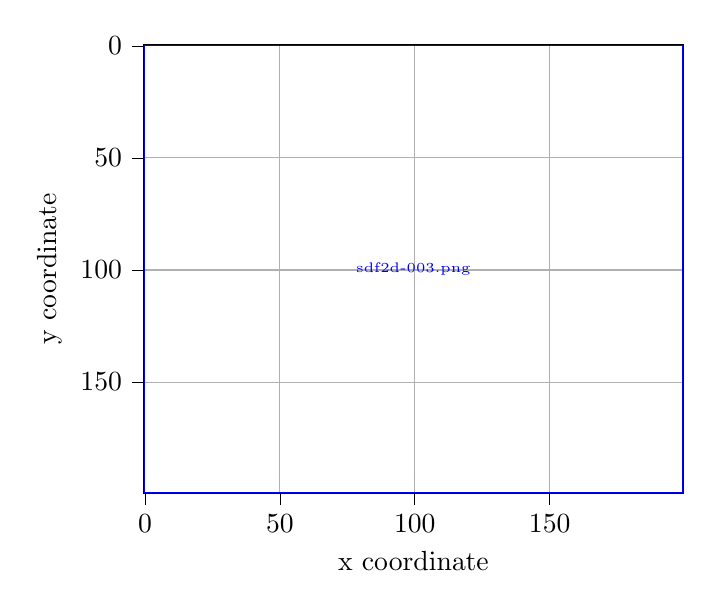
\begin{tikzpicture}

\begin{axis}[
tick align=outside,
tick pos=left,
x grid style={white!69.0196!black},
xlabel={x coordinate},
xmajorgrids,
xmin=-0.5000, xmax=199.5000,
xtick style={color=black},
y dir=reverse,
y grid style={white!69.0196!black},
ylabel={y coordinate},
ymajorgrids,
ymin=-0.5000, ymax=199.5000,
ytick style={color=black}
]
\addplot graphics [includegraphics cmd=\pgfimage,xmin=-0.5000, xmax=199.5000, ymin=199.5000, ymax=-0.5000] {sdf2d-003.png};
\end{axis}

\end{tikzpicture}

        % % This file was created by tikzplotlib v0.9.1.
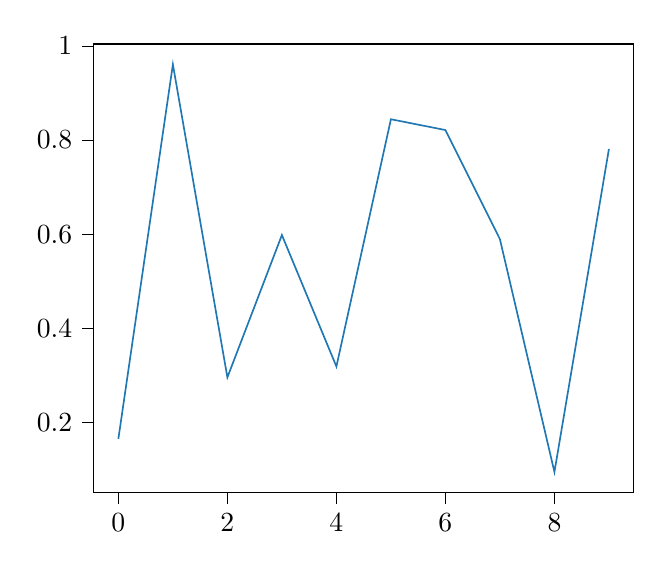
\begin{tikzpicture}

\definecolor{color0}{rgb}{0.12156862745098,0.466666666666667,0.705882352941177}

\begin{axis}[
tick align=outside,
tick pos=left,
x grid style={white!69.0196078431373!black},
xmin=-0.45, xmax=9.45,
xtick style={color=black},
y grid style={white!69.0196078431373!black},
ymin=0.0515297644926165, ymax=1.0037743262763,
ytick style={color=black}
]
\addplot [semithick, color0]
table {%
0 0.165204368712852
1 0.960490482558861
2 0.295706783168825
3 0.598084081751131
4 0.318814100655487
5 0.844017623549353
6 0.821076195130074
7 0.589191813076777
8 0.0948136082100567
9 0.781036863745426
};
\end{axis}

\end{tikzpicture}

    \end{center}
    \caption{a two dimensional SDF. $F(x,y) = \sqrt{x^2+y^2} - 1$} describes the unit circle.
\end{figure}

Since the distance to the nearest surface is always known, the step size of a ray tracing algorithm can be dynamically adjusted, resulting in fewer iterations along a ray, see figure

% This enables the technique of sphere tracing, which has been used extensively in the so called demo scene to render impressive 3D video demos in real time for decades. 


% \begin{figure}[ht]
% \centerline{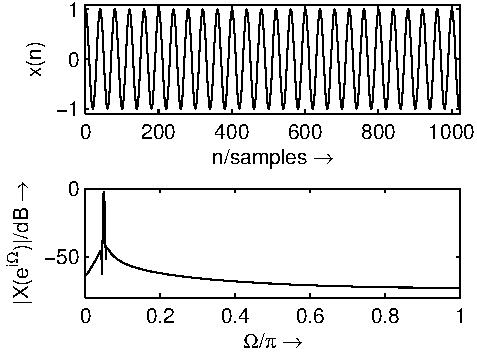
\includegraphics[scale=0.8]{fft_plot2}}
% \caption{\label{fft_plot}{\it Sinusoid in time and frequency domain. Short captions are centred, long captions (more than 1 line) are justified.}}
% \end{figure}


\subsection{Previous Work}
\label{ssec:prev}

As shown in \cite{brinkmann_round_2019} there exist multiple approaches for estimating RIRs.  
NVIDIA is working in the field of real time ray traced audio simulation
NVIDIA VRWorks™ Audio (introduced with the Pascal GPU architecture) 

\cite{cao_interactive_2016} bidirectional raytracing.

\subsubsection*{RIR Estimation}
image sourcce method, wave based, raytracing.


\subsubsection*{Sphere Tracing}

Defining SDFs is an active field of research and there are several projects that aim at easier construction of SDFs and integration in 3D frameworks such as \href{https://github.com/Flafla2/Generic-Raymarch-Unity}{https://github.com/Flafla2/Generic-Raymarch-Unity} and \cite{lechner_hrtlacektdraymarchtoolkit_2020}.



\subsection{Motivation}
The reasons why sphere tracing in a compute shader for RIR estimation has not been documented until now probably lie in the relatively new introduction of compute shaders as well as in the difficulty of creating SDFs(in comparison to using existing 3D /CAD models and import them to polygon based ray tracers).
\subsubsection{Sphere tracing}
As described above, ray tracing in general is in use.
procedural by default
deforming geometry
\subsubsection{Implementation}
It is possible to implement the chosen algorithm on the CPU and the GPU. A number of frameworks could be chosen for GPU accelerated computation such as OpenCL or NVIDIA CUDA. The choice of a shader has the advantage of being more operating system independent and hardware independent. Compute shaders (in contrast to fragment shaders) make it possible to write to arbitrary output locations which is necessary for generating the actual impulse response from the measurement of timings. Since they are available since OpenGL 4.3 (August 2012) / OpenGL ES 3.1 they are both old enough have received broad support in other frameworks and relatively new in respect to first publications about sphere tracing. Another reason for the choice of compute shaders is their simplicity. In comparison to CUDA and OpenCL, shaders are easier to write and the GLSL(Graphics Library Shading Language) is more widespread. 


\section{Generation of SDFs}

\section{Sphere Tracing}
For simplicity, deterministic equal-angle Ray Tracing is used in contrast to Monte Carlo or Equal Area Ray tracing (EART) \cite{gu_room_2014}.

low frequency pass

\section{Generation of impulse response}

Advantage of compute shader.
Maybe introduce cascaded Lowpass.



All figures should be centred on the column (or page, if the figure spans both columns).
Figure captions (in italic) should follow each figure and have the format given in Figure \ref{fft_plot}.
%
Vectorial figures are preferred. For example when using
\texttt{Matlab}, export using either Postscript or PDF format. Also,
in order to provide a better readability, figure text font size
should be at least identical to footnote font size. To do so using
\texttt{Matlab}, use the \texttt{subplot} command before plotting.
If bitmap figures are used, please make sure that the resolution is
enough for print quality. Fig. \ref{ftt_plot2} illustrates an
example of a figure spanning two columns.
%

\section{Results}

compare to \cite{brinkmann_round_2019}
compare to \cite{campbell_roomsim_nodate}


\begin{figure}[ht]
\centerline{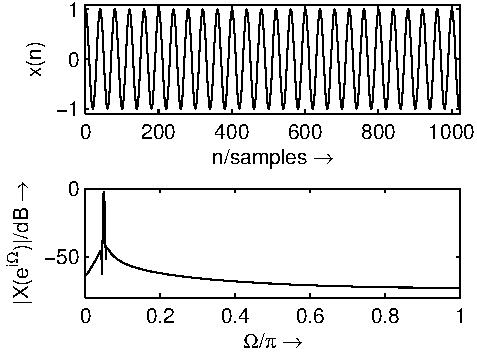
\includegraphics[scale=0.8]{fft_plot2}}
\caption{\label{fft_plot}{\it Sinusoid in time and frequency domain. Short captions are centred, long captions (more than 1 line) are justified.}}
\end{figure}
%
\begin{figure*}[ht]
\center
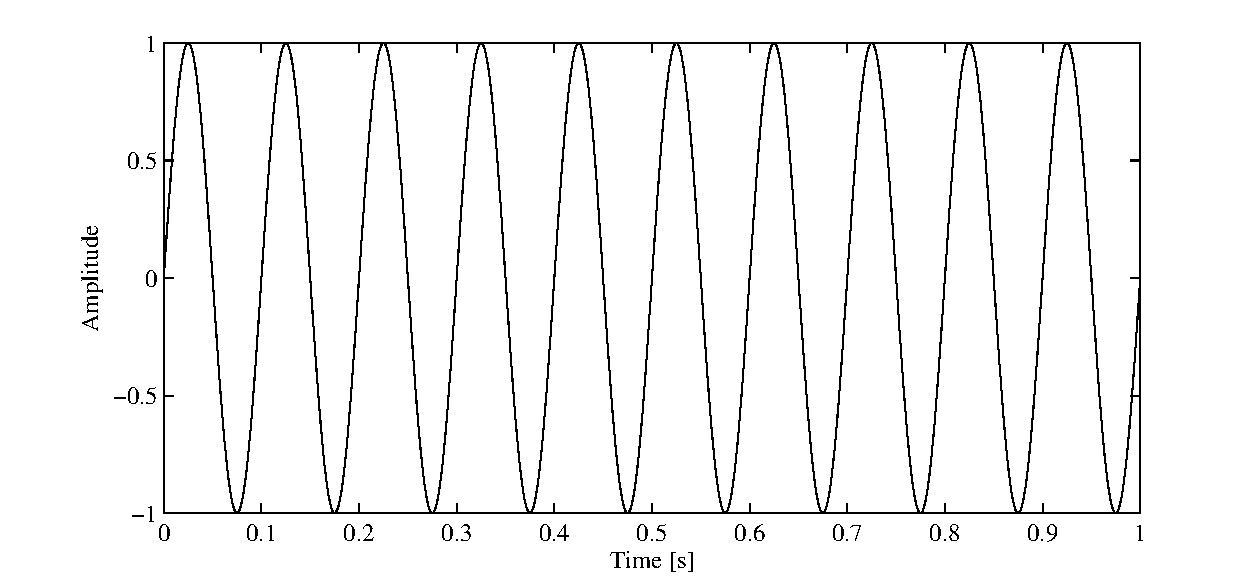
\includegraphics[width=5in]{TwoColumnSine2}
\caption{\label{ftt_plot2}{\it A figure spanning two columns, as mentioned in Sec. . }}
\end{figure*}


% \begin{figure}[ht]
% \centerline{\includegraphics[scale=0.8]{img/test1.pgf}}
% \caption{\label{fft_plot}{\it Sinusoid in time and frequency domain. Short captions are centred, long captions (more than 1 line) are justified.}}
% \end{figure}

\begin{figure}
    \begin{center}
      % This file was created by tikzplotlib v0.9.1.
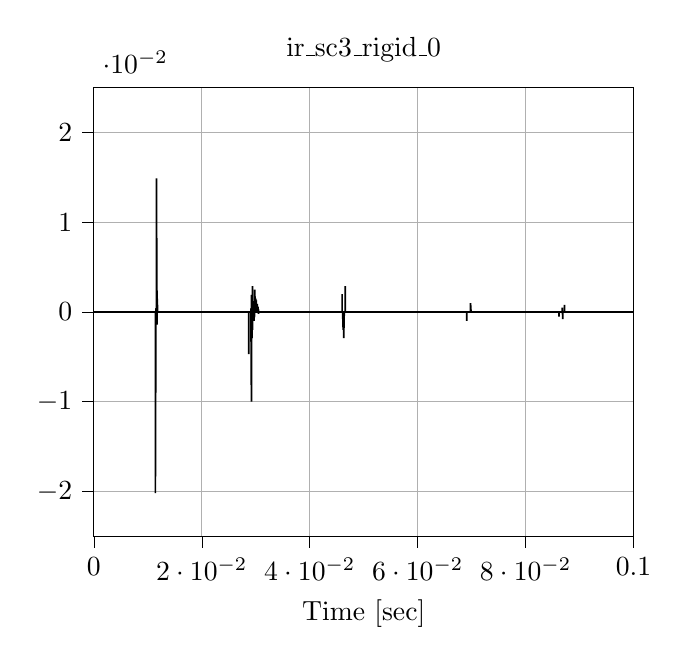
\begin{tikzpicture}

\begin{axis}[
tick align=outside,
tick pos=left,
title={ir\_sc3\_rigid\_0},
x grid style={white!69.0196!black},
xlabel={Time [sec]},
xmajorgrids,
xmin=0.0000, xmax=0.1000,
xtick style={color=black},
y grid style={white!69.0196!black},
ymajorgrids,
ymin=-0.0250, ymax=0.0250,
ytick style={color=black}
]
\addplot [semithick, black]
table {%
0.0000 0.0000
0.0114 0.0000
0.0114 -0.0202
0.0115 0.0000
0.0115 0.0000
0.0115 0.0000
0.0115 0.0001
0.0116 0.0000
0.0116 0.0001
0.0116 0.0149
0.0117 -0.0014
0.0117 0.0024
0.0117 0.0003
0.0117 0.0020
0.0118 0.0005
0.0118 0.0000
0.0121 0.0000
0.0287 0.0000
0.0287 -0.0047
0.0287 0.0000
0.0291 0.0000
0.0291 0.0004
0.0292 -0.0100
0.0292 0.0019
0.0292 -0.0009
0.0292 -0.0006
0.0293 0.0004
0.0293 -0.0001
0.0293 -0.0000
0.0293 0.0004
0.0293 -0.0029
0.0294 0.0029
0.0294 -0.0020
0.0294 0.0018
0.0295 -0.0001
0.0295 0.0000
0.0295 0.0009
0.0295 -0.0009
0.0295 0.0012
0.0296 -0.0004
0.0296 0.0000
0.0296 -0.0005
0.0297 0.0010
0.0297 -0.0010
0.0297 0.0011
0.0297 -0.0008
0.0298 0.0013
0.0298 -0.0005
0.0298 0.0025
0.0299 0.0009
0.0299 0.0012
0.0299 0.0007
0.0300 0.0011
0.0300 0.0007
0.0300 -0.0001
0.0300 0.0015
0.0300 0.0005
0.0301 0.0007
0.0301 0.0004
0.0301 0.0008
0.0302 0.0004
0.0302 0.0008
0.0302 0.0002
0.0302 0.0007
0.0303 0.0006
0.0303 -0.0001
0.0303 0.0009
0.0303 -0.0000
0.0304 0.0006
0.0304 0.0004
0.0304 0.0000
0.0304 0.0006
0.0305 -0.0002
0.0305 0.0003
0.0305 0.0000
0.0460 0.0000
0.0460 0.0020
0.0460 -0.0000
0.0461 -0.0000
0.0462 -0.0020
0.0462 0.0000
0.0463 0.0000
0.0463 -0.0029
0.0464 -0.0000
0.0465 0.0000
0.0466 0.0000
0.0466 0.0029
0.0466 0.0000
0.0691 0.0000
0.0691 -0.0010
0.0691 0.0000
0.0698 0.0000
0.0698 0.0010
0.0699 0.0000
0.0862 0.0000
0.0862 -0.0005
0.0862 0.0000
0.0868 0.0000
0.0868 0.0005
0.0869 -0.0008
0.0869 0.0000
0.0872 0.0000
0.0872 0.0008
0.0872 0.0000
0.1000 0.0000
};
\end{axis}

\end{tikzpicture}

        % % This file was created by tikzplotlib v0.9.1.
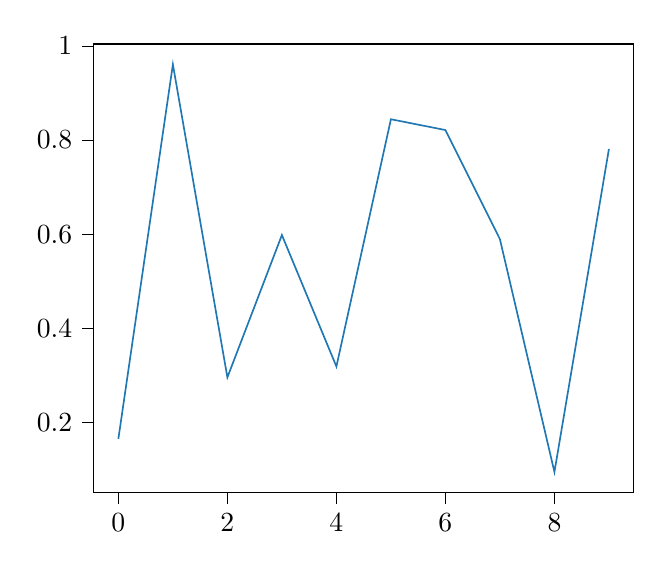
\begin{tikzpicture}

\definecolor{color0}{rgb}{0.12156862745098,0.466666666666667,0.705882352941177}

\begin{axis}[
tick align=outside,
tick pos=left,
x grid style={white!69.0196078431373!black},
xmin=-0.45, xmax=9.45,
xtick style={color=black},
y grid style={white!69.0196078431373!black},
ymin=0.0515297644926165, ymax=1.0037743262763,
ytick style={color=black}
]
\addplot [semithick, color0]
table {%
0 0.165204368712852
1 0.960490482558861
2 0.295706783168825
3 0.598084081751131
4 0.318814100655487
5 0.844017623549353
6 0.821076195130074
7 0.589191813076777
8 0.0948136082100567
9 0.781036863745426
};
\end{axis}

\end{tikzpicture}

    \end{center}
    \caption{A PGF histogram from \texttt{matplotlib}.}
\end{figure}




\subsection{Tables}
As for figures, all tables should be centered on the column (or page, if the table spans both columns).
Table captions should be in italic, precede each table and have the format given in Table \ref{tab:example}.

\begin{table}[ht]
  \caption{\itshape Basic trigonometric values.}
	\centering
	\begin{tabular}{|c|c|}
		\hline
		$\mathrm{angle}\,(\theta, \mathrm{rad})$ & $\sin \theta$ \\\hline
		$\frac{\pi}{2}$ & $1$ \\
		$\pi$ & $0$ \\
		$\frac{3\pi}{2}$ & $-1$ \\
		$2\pi$ & $0$ \\\hline
	\end{tabular}
	%
	\label{tab:example}
\end{table}

\begin{table*}[ht]
  \caption{{\it Basic trigonometric values, spanning two columns.}}
	\centering
  \begin{tabular}{|c|c|c|c|c|c|c|}\hline
    $\mathrm{angle}\, (\theta, \mathrm{rad})$ & $\sin \theta$ & $\cos \theta $ & $(\sin \theta)/2 $ & $(\cos \theta) /2 $ & $(\sin \theta)/3 $ & $(\cos \theta)/3$    \\\hline
    $\frac{\pi}{2}$ & $1$ & $0$ & $1/2$ & $0$ & $1/3$ & $0$ \\
    $\pi$ & $0$ & $-1$ & $0$ & $-1/2$ & $0$ & $-1/3$\\
    $\frac{3\pi}{2}$ & $-1$ & $0$ & $-1/2$ & $0$ & $-1/3$ & $0$ \\
    $2\pi$ & $0$ & $1$ & $0$ & $1/2$ & $0$ & $1/3$ \\\hline
 \end{tabular}
	%
  \label{tab:example2}
\end{table*}

\subsection{Equations}
Equations should be placed on separate lines and numbered:

\begin{equation}
	X(e^{j\Omega})=\sum_{n=0}^{N-1}x(n)e^{-j\Omega n}
	\label{eq1}
	\end{equation}
	where the sequence $x(n)$ in equation (\ref{eq1}) is a windowed frame:
	\begin{equation}
	x(n)=s(n) w(n)
	\label{eq2}
\end{equation}
%
with a window function $w(n)$.


\subsection{Page Numbers}
Page numbers will be added to the document in the postprocessing stage, so {\em please leave the numbering as is},
that is, the first page will start at page DAFX-1 and the last page, at most, will have to be DAFX-8.


\subsection{References}
% The references will be numbered in order of appearance \cite{Mitra:Kaiser:1993:DSP:handbook}, \cite{Haykin:1991:adaptive:filter}, \cite{Moorer:2000:AES:audio:millenium} and \cite{Nackaerts:2001:ICMC}. Please avoid listing references that do not appear in the text (we did the opposite in this template).


\subsubsection{Reference Format}
The reference format is the standard IEEE one. We recommend to use BibTeX to create the reference list.


\section{Conclusions}
This template can be found on the conference website.
For changing the number of author affiliations (1 to 4), uncomment the corresponding regions in the template \texttt{tex} file.
Please, submit full-length papers (max.~8 pages both oral and poster presentations).
Submission is fully electronic and automated through the Conference Web Submission System.
DO NOT send us papers directly by e-mail.

\section{Acknowledgments}
Many thanks to the great number of anonymous reviewers!

%\newpage
\nocite{*}
\bibliographystyle{IEEEbib}
% \bibliography{DAFx20_tmpl} % requires file DAFx20_tmpl.bib
\bibliography{RaymarchReverb2}


\section{Appendix: Margin Check}
This section shows the column margins for the text. \bigskip\newline

Lorem ipsum dolor sit amet, consectetur adipisici elit, sed eiusmod tempor incidunt ut labore et dolore magna aliqua. Ut enim ad minim veniam, quis nostrud exercitation ullamco laboris nisi ut aliquid ex ea commodi consequat. Quis aute iure reprehenderit in voluptate velit esse cillum dolore eu fugiat nulla pariatur. Excepteur sint obcaecat cupiditat non proident, sunt in culpa qui officia deserunt mollit anim id est laborum.


Duis autem vel eum iriure dolor in hendrerit in vulputate velit esse molestie consequat, vel illum dolore eu feugiat nulla facilisis at vero eros et accumsan et iusto odio dignissim qui blandit praesent luptatum zzril delenit augue duis dolore te feugait nulla facilisi. Lorem ipsum dolor sit amet, consectetuer adipiscing elit, sed diam nonummy nibh euismod tincidunt ut laoreet dolore magna aliquam erat volutpat.

Ut visi enim ad minim veniam, quis nostrud exerci tation ullamcorper suscipit lobortis nisl ut aliquip ex ea commodo consequat. Duis autem vel eum iriure dolor in hendrerit in vulputate velit esse molestie consequat, vel illum dolore eu feugiat nulla facilisis at vero eros et accumsan et iusto odio dignissim qui blandit praesent luptatum zzril delenit augue duis dolore te feugait nulla facilisi.

Nam liber tempor cum soluta nobis eleifend option congue nihil imperdiet doming id quod mazim placerat facer possim assum. Lorem ipsum dolor sit amet, consectetuer adipiscing elit, sed diam nonummy nibh euismod tincidunt ut laoreet dolore magna aliquam erat volutpat. Ut wisi enim ad minim veniam, quis nostrud exerci tation ullamcorper suscipit lobortis nisl ut aliquip ex ea commodo consequat.

Duis autem vel eum iriure dolor in hendrerit in vulputate velit esse molestie consequat, vel illum dolore eu feugiat nulla facilisis.

At vero eos et accusam et justo duo dolores et ea rebum. Stet clita kasd gubergren, no sea takimata sanctus est Lorem ipsum dolor sit amet. Lorem ipsum dolor sit amet, consetetur sadipscing elitr, sed diam nonumy eirmod tempor invidunt ut labore et dolore magna aliquyam erat, sed diam voluptua. At vero eos et accusam et justo duo dolores et ea rebum. Stet clita kasd gubergren, no sea takimata sanctus est Lorem ipsum dolor sit amet. Lorem ipsum dolor sit amet, consetetur sadipscing elitr, At accusam aliquyam diam diam dolore dolores duo eirmod eos erat, et nonumy sed tempor et et invidunt justo labore Stet clita ea et gubergren, kasd magna no rebum. sanctus sea sed takimata ut vero voluptua. est Lorem ipsum dolor sit amet. Lorem ipsum dolor sit amet, consetetur sadipscing elitr, sed diam nonumy eirmod tempor invidunt ut labore et dolore magna aliquyam erat.

Consetetur sadipscing elitr, sed diam nonumy eirmod tempor invidunt ut labore et dolore magna aliquyam erat, sed diam voluptua. At vero eos et accusam et justo duo dolores et ea rebum. Stet clita kasd gubergren, no sea takimata sanctus est Lorem ipsum dolor sit amet. Lorem ipsum dolor sit amet, consetetur sadipscing elitr, sed diam nonumy eirmod tempor invidunt ut labore et dolore magna aliquyam erat, sed diam voluptua. At vero eos et accusam et justo duo dolores et ea rebum. Stet clita kasd gubergren, no sea takimata sanctus est Lorem ipsum dolor sit amet. Lorem ipsum dolor sit amet, consetetur sadipscing elitr, sed diam nonumy eirmod tempor invidunt ut labore et dolore magna aliquyam erat, sed diam voluptua. At vero eos et accusam et justo duo dolores et ea rebum. Stet clita kasd gubergren, no sea takimata sanctus est Lorem ipsum dolor sit amet.

Lorem ipsum dolor sit amet, consectetur adipisici elit, sed eiusmod tempor incidunt ut labore et dolore magna aliqua. Ut enim ad minim veniam, quis nostrud exercitation ullamco laboris nisi ut aliquid ex ea commodi consequat. Quis aute iure reprehenderit in voluptate velit esse cillum dolore eu fugiat nulla pariatur. Excepteur sint obcaecat cupiditat non proident, sunt in culpa qui officia deserunt mollit anim id est laborum.


Duis autem vel eum iriure dolor in hendrerit in vulputate velit esse molestie consequat, vel illum dolore eu feugiat nulla facilisis at vero eros et accumsan et iusto odio dignissim qui blandit praesent luptatum zzril delenit augue duis dolore te feugait nulla facilisi. Lorem ipsum dolor sit amet, consectetuer adipiscing elit, sed diam nonummy nibh euismod tincidunt ut laoreet dolore magna aliquam erat volutpat.

Ut wisi enim ad minim veniam, quis nostrud exerci tation ullamcorper suscipit lobortis nisl ut aliquip ex ea commodo consequat. Duis autem vel eum iriure dolor in hendrerit in vulputate velit esse molestie consequat, vel illum dolore eu feugiat nulla facilisis at vero eros et accumsan et iusto odio dignissim qui blandit praesent luptatum zzril delenit augue duis dolore te feugait nulla facilisi.

Nam liber tempor cum soluta nobis eleifend option congue nihil imperdiet doming id quod mazim placerat facer possim assum. Lorem ipsum dolor sit amet, consectetuer adipiscing elit, sed diam nonummy nibh euismod tincidunt ut laoreet dolore magna aliquam erat volutpat. Ut wisi enim ad minim veniam, quis nostrud exerci tation ullamcorper suscipit lobortis nisl ut aliquip ex ea commodo consequat.

Duis autem vel eum iriure dolor in hendrerit in vulputate velit esse molestie consequat, vel illum dolore eu feugiat nulla facilisis.

At vero eos et accusam et justo duo dolores et ea rebum. Stet clita kasd gubergren, no sea takimata sanctus est Lorem ipsum dolor sit amet. Lorem ipsum dolor sit amet, consetetur sadipscing elitr, sed diam nonumy eirmod tempor invidunt ut labore et dolore magna aliquyam erat, sed diam voluptua. At vero eos et accusam et justo duo dolores et ea rebum. Stet clita kasd gubergren, no sea takimata sanctus est Lorem ipsum dolor sit amet. Lorem ipsum dolor sit amet, consetetur sadipscing elitr, At accusam aliquyam diam diam dolore dolores duo eirmod eos erat, et nonumy sed tempor et et invidunt justo labore Stet clita ea et gubergren, kasd magna no rebum. sanctus sea sed takimata ut vero voluptua. est Lorem ipsum dolor sit amet. Lorem ipsum dolor sit amet, consetetur sadipscing elitr, sed diam nonumy eirmod tempor invidunt ut labore et dolore magna aliquyam erat.

Consetetur sadipscing elitr, sed diam nonumy eirmod tempor invidunt ut labore et dolore magna aliquyam erat, sed diam voluptua. At vero eos et accusam et justo duo dolores et ea rebum. Stet clita kasd gubergren, no sea takimata sanctus est Lorem ipsum dolor sit amet. Lorem ipsum dolor sit amet, consetetur sadipscing elitr, sed diam nonumy eirmod tempor invidunt ut labore et dolore magna aliquyam erat, sed diam voluptua. At vero eos et accusam et justo duo dolores et ea rebum. Stet clita kasd gubergren, no sea takimata sanctus est Lorem ipsum dolor sit amet. 

Lorem ipsum dolor sit amet, consectetur adipisici elit, sed eiusmod tempor incidunt ut labore et dolore magna aliqua. Ut enim ad minim veniam, quis nostrud exercitation ullamco laboris nisi ut aliquid ex ea commodi consequat. Quis aute iure reprehenderit in voluptate velit esse cillum dolore eu fugiat nulla pariatur. Excepteur sint obcaecat cupiditat non proident, sunt in culpa qui officia deserunt mollit anim id est laborum.

%%Duis autem vel eum iriure dolor in hendrerit in vulputate velit esse molestie consequat, vel illum dolore eu feugiat nulla facilisis at vero eros et accumsan et iusto odio dignissim qui blandit praesent luptatum zzril delenit augue duis dolore te feugait nulla facilisi. Lorem ipsum dolor sit amet, consectetuer adipiscing elit, sed diam nonummy nibh euismod tincidunt ut laoreet dolore magna aliquam erat volutpat.

%%Ut visi enim ad minim veniam, quis nostrud exerci tation ullamcorper suscipit lobortis nisl ut aliquip ex ea commodo consequat. Duis autem vel eum iriure dolor in hendrerit in vulputate velit esse molestie consequat, vel illum dolore eu feugiat nulla facilisis at vero eros et accumsan et iusto odio dignissim qui blandit praesent luptatum zzril delenit augue duis dolore te feugait nulla ..
\end{document}
